% Choose one to switch between slides and handout
\documentclass[]{beamer}
%\documentclass[handout]{beamer}

% Video Meta Data
\title{Bitcoin, Blockchain and Cryptoassets}
\subtitle{History of Digital Money}
\author{Prof. Dr. Fabian Schär}
\institute{University of Basel}

% Config File
% Packages
\usepackage[utf8]{inputenc} 
\usepackage{hyperref}
\usepackage{gitinfo2}
\usepackage{tikz}
\usepackage{amsmath}
\usepackage{bibentry}
\usepackage{xcolor}
\usepackage{caption}

% Beamer Template Options
\beamertemplatenavigationsymbolsempty
\setbeamertemplate{footline}[frame number]
\setbeamercolor{structure}{fg=black}
\setbeamercolor{footline}{fg=black}
\setbeamercolor{title}{fg=black}
\setbeamercolor{frametitle}{fg=black}
\setbeamercolor{item}{fg=black}
\setbeamercolor{}{fg=black}
\setbeamercolor{bibliography item}{fg=black}
\setbeamercolor*{bibliography entry title}{fg=black}
\setbeamertemplate{items}[square]
\setbeamertemplate{enumerate items}[default]
\captionsetup[figure]{labelfont={color=black},font={color=black}}
\captionsetup[table]{labelfont={color=black},font={color=black}}

\setbeamertemplate{bibliography item}{\insertbiblabel}

% Link Icon Command
\newcommand{\link}{%
    \tikz[x=1.2ex, y=1.2ex, baseline=-0.05ex]{% 
        \begin{scope}[x=1ex, y=1ex]
            \clip (-0.1,-0.1) 
                --++ (-0, 1.2) 
                --++ (0.6, 0) 
                --++ (0, -0.6) 
                --++ (0.6, 0) 
                --++ (0, -1);
            \path[draw, 
                line width = 0.5, 
                rounded corners=0.5] 
                (0,0) rectangle (1,1);
        \end{scope}
        \path[draw, line width = 0.5] (0.5, 0.5) 
            -- (1, 1);
        \path[draw, line width = 0.5] (0.6, 1) 
            -- (1, 1) -- (1, 0.6);
        }
    }

% Custom Titlepage
\defbeamertemplate*{title page}{customized}[1][]
{
  \vspace{-0cm}\hfill\includegraphics[width=2.5cm]{../config/logo_cif} 
  \includegraphics[width=1.9cm]{../config/seal_wwz} 
  \\ \vspace{2em}
  \usebeamerfont{title}\textbf{\inserttitle}\par
  \usebeamerfont{title}\usebeamercolor[fg]{title}\insertsubtitle\par  \vspace{1.5em}
  \small\usebeamerfont{author}\insertauthor\par
  \usebeamerfont{author}\insertinstitute\par \vspace{2em}
  \usebeamercolor[fg]{titlegraphic}\inserttitlegraphic
    \tiny \noindent \texttt{Commit Hash: \gitHash}\\ 
	\texttt{Commit Time: \gitAuthorIsoDate}\\ \vspace{1em}
  \link \href{https://github.com/cifunibas/Bitcoin-Blockchain-Cryptoassets/blob/main/slides/intro.pdf}
  {Get most recent version}\\
  \link \href{https://github.com/cifunibas/Bitcoin-Blockchain-Cryptoassets/blob/main/slides/intro.pdf}
  {Watch video lecture}\\ \vspace{1em}
  License: \texttt{Creative Commons Attribution-NonCommercial-ShareAlike 4.0 International}\\\vspace{2em}
  \includegraphics[width = 1.2cm]{../config/license}
}


%%%%%%%%%%%%%%%%%%%%%%%%%%%%%%%%%%%%%%%%%%%%%%
%%%%%%%%%%%%%%%%%%%%%%%%%%%%%%%%%%%%%%%%%%%%%%
\begin{document}

\thispagestyle{empty}
\begin{frame}[noframenumbering]
	\titlepage
\end{frame}



%%%
\begin{frame}{Before Bitcoin}
\begin{columns}
	\column{0.4\textwidth}
		\begin{figure}
			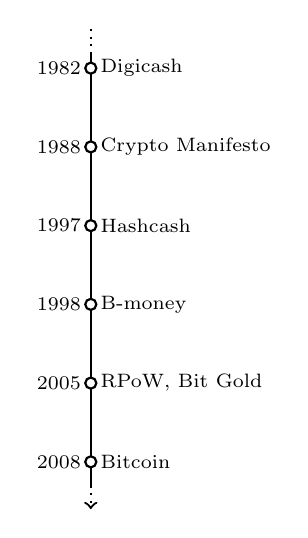
\begin{tikzpicture}[scale=1]
						%draw vertical line
		%\draw [thick] (0,4) -- (0,2.3);
		%\draw [thick,dotted] (0,2.3) -- (0,1.7);
		%\draw [thick] (0,1.7) -- (0,0.3);
		%\draw [thick,dotted] (0,0.3) -- (0,-0.3);
		%\draw [thick, ->] (0,-0.3) -- (0,-2);
		\draw [thick,dotted] (0,4) -- (0,3.7);
		\draw [thick] (0,3.7) -- (0,-1.8);
		\draw [thick,dotted, ->] (0,-1.8) -- (0,-2.1);
		
		%draw bullet points
		\foreach \x in {3.5,2.5,1.5,0.5,-0.5,-1.5}
		\filldraw[draw=black, fill = white, thick] (0, \x cm) circle (2pt);
		
		
		%years & names
		\draw(0,3.5) node[left] {{\scriptsize 1982}} node[right] {{\scriptsize Digicash}};
		\draw(0,2.5) node[left] {{\scriptsize 1988}} node[right] {{\scriptsize Crypto Manifesto}};
		\draw(0,1.5) node[left] {{\scriptsize 1997}} node[right] {{\scriptsize Hashcash}};
		\draw(0,0.5) node[left] {{\scriptsize 1998}} node[right] {{\scriptsize B-money}};
		\draw(0,-0.5) node[left] {{\scriptsize 2005}} node[right] {{\scriptsize RPoW, Bit Gold}};
		\draw(0,-1.5) node[left] {{\scriptsize 2008}} node[right] {{\scriptsize Bitcoin}};
	
			\end{tikzpicture}
		\end{figure}
	\column{0.7\textwidth}
		\textbf{Digicash - David Chaum}
		\vspace{0.5em}
		\begin{small}
		\begin{itemize}
			\item Electronic means of payment significantly limit privacy and traceable payment flows generate sensitive data.
			\item Goal: Virtual money unit that imitates the anonymity of cash.
			\item Monopolized money creation and centralized settlement.
			\item Central bank blindly signs money units.
		\end{itemize}
		\end{small}	
\end{columns}
\end{frame}
%%%



%%%
\begin{frame}{Before Bitcoin}
\begin{columns}
\column{0.4\textwidth}
\begin{figure}
	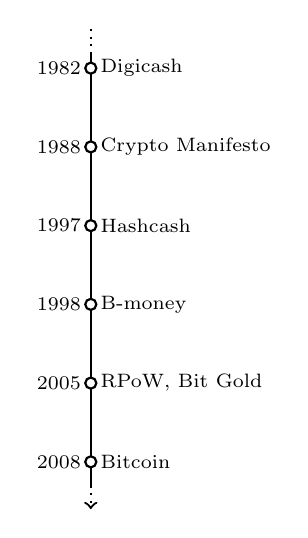
\begin{tikzpicture}[scale=1]
				%draw vertical line
		%\draw [thick] (0,4) -- (0,2.3);
		%\draw [thick,dotted] (0,2.3) -- (0,1.7);
		%\draw [thick] (0,1.7) -- (0,0.3);
		%\draw [thick,dotted] (0,0.3) -- (0,-0.3);
		%\draw [thick, ->] (0,-0.3) -- (0,-2);
		\draw [thick,dotted] (0,4) -- (0,3.7);
		\draw [thick] (0,3.7) -- (0,-1.8);
		\draw [thick,dotted, ->] (0,-1.8) -- (0,-2.1);
		
		%draw bullet points
		\foreach \x in {3.5,2.5,1.5,0.5,-0.5,-1.5}
		\filldraw[draw=black, fill = white, thick] (0, \x cm) circle (2pt);
		
		
		%years & names
		\draw(0,3.5) node[left] {{\scriptsize 1982}} node[right] {{\scriptsize Digicash}};
		\draw(0,2.5) node[left] {{\scriptsize 1988}} node[right] {{\scriptsize Crypto Manifesto}};
		\draw(0,1.5) node[left] {{\scriptsize 1997}} node[right] {{\scriptsize Hashcash}};
		\draw(0,0.5) node[left] {{\scriptsize 1998}} node[right] {{\scriptsize B-money}};
		\draw(0,-0.5) node[left] {{\scriptsize 2005}} node[right] {{\scriptsize RPoW, Bit Gold}};
		\draw(0,-1.5) node[left] {{\scriptsize 2008}} node[right] {{\scriptsize Bitcoin}};
	
	\end{tikzpicture}
\end{figure}
\column{0.7\textwidth}
	\textbf{Hashcash - Adam Back}
	\vspace{0.5em}
	\begin{small}
	\begin{itemize}
		\item Originally proposed as a mechanism for anti-DoS and spam email.
		\item Introduced concept of artificial costs.
		\item "The idea of using partial hashes is that they can be made arbitrarily expensive to compute (by choosing the desired number of bits of collision), and yet can be verified instantly."
	\end{itemize}
	\end{small}
\end{columns}
\end{frame}
%%%	


%%%
\begin{frame}{Before Bitcoin}
\begin{columns}
\column{0.4\textwidth}
\begin{figure}
	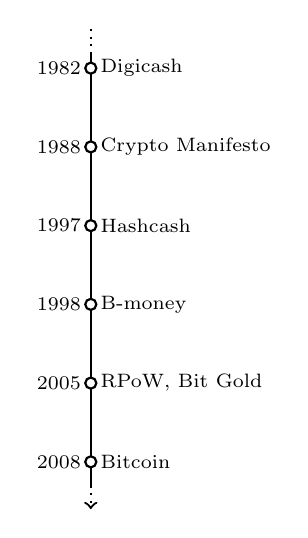
\begin{tikzpicture}[scale=1]
				%draw vertical line
		%\draw [thick] (0,4) -- (0,2.3);
		%\draw [thick,dotted] (0,2.3) -- (0,1.7);
		%\draw [thick] (0,1.7) -- (0,0.3);
		%\draw [thick,dotted] (0,0.3) -- (0,-0.3);
		%\draw [thick, ->] (0,-0.3) -- (0,-2);
		\draw [thick,dotted] (0,4) -- (0,3.7);
		\draw [thick] (0,3.7) -- (0,-1.8);
		\draw [thick,dotted, ->] (0,-1.8) -- (0,-2.1);
		
		%draw bullet points
		\foreach \x in {3.5,2.5,1.5,0.5,-0.5,-1.5}
		\filldraw[draw=black, fill = white, thick] (0, \x cm) circle (2pt);
		
		
		%years & names
		\draw(0,3.5) node[left] {{\scriptsize 1982}} node[right] {{\scriptsize Digicash}};
		\draw(0,2.5) node[left] {{\scriptsize 1988}} node[right] {{\scriptsize Crypto Manifesto}};
		\draw(0,1.5) node[left] {{\scriptsize 1997}} node[right] {{\scriptsize Hashcash}};
		\draw(0,0.5) node[left] {{\scriptsize 1998}} node[right] {{\scriptsize B-money}};
		\draw(0,-0.5) node[left] {{\scriptsize 2005}} node[right] {{\scriptsize RPoW, Bit Gold}};
		\draw(0,-1.5) node[left] {{\scriptsize 2008}} node[right] {{\scriptsize Bitcoin}};
	
	\end{tikzpicture}
\end{figure}
\column{0.7\textwidth}
	\textbf{B-money - Wei Dai} \\
	\vspace{0.5em}
	\begin{small}
	\begin{itemize}
		\item Thought experiment
		\item Assumption: Existence of an untraceable network.
		\item Senders and receivers are identified only by digital pseudonyms. (i.e. public keys) 
		\item Transaction legitimacy guaranteed by signature with associated private key.
		\item Participants keep separate registers with the current balances of all pseudonyms.
		\item Competitive money creation by solving numerical puzzles that are hard to compute but easy to verify.
	\end{itemize}
	\end{small}
\end{columns}
\end{frame}
%%%	


%%%
\begin{frame}{Before Bitcoin}
\begin{columns}
\column{0.4\textwidth}
\begin{figure}
	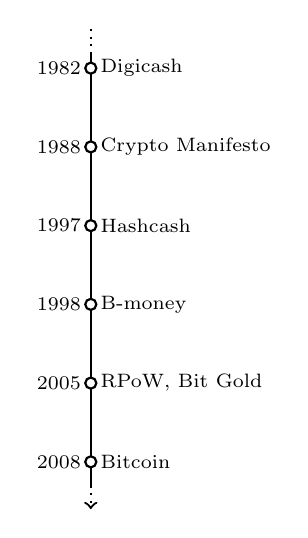
\begin{tikzpicture}[scale=1]
				%draw vertical line
		%\draw [thick] (0,4) -- (0,2.3);
		%\draw [thick,dotted] (0,2.3) -- (0,1.7);
		%\draw [thick] (0,1.7) -- (0,0.3);
		%\draw [thick,dotted] (0,0.3) -- (0,-0.3);
		%\draw [thick, ->] (0,-0.3) -- (0,-2);
		\draw [thick,dotted] (0,4) -- (0,3.7);
		\draw [thick] (0,3.7) -- (0,-1.8);
		\draw [thick,dotted, ->] (0,-1.8) -- (0,-2.1);
		
		%draw bullet points
		\foreach \x in {3.5,2.5,1.5,0.5,-0.5,-1.5}
		\filldraw[draw=black, fill = white, thick] (0, \x cm) circle (2pt);
		
		
		%years & names
		\draw(0,3.5) node[left] {{\scriptsize 1982}} node[right] {{\scriptsize Digicash}};
		\draw(0,2.5) node[left] {{\scriptsize 1988}} node[right] {{\scriptsize Crypto Manifesto}};
		\draw(0,1.5) node[left] {{\scriptsize 1997}} node[right] {{\scriptsize Hashcash}};
		\draw(0,0.5) node[left] {{\scriptsize 1998}} node[right] {{\scriptsize B-money}};
		\draw(0,-0.5) node[left] {{\scriptsize 2005}} node[right] {{\scriptsize RPoW, Bit Gold}};
		\draw(0,-1.5) node[left] {{\scriptsize 2008}} node[right] {{\scriptsize Bitcoin}};
	
	\end{tikzpicture}
\end{figure}
\column{0.7\textwidth}
	\textbf{Reusable Proofs of Work - Hal Finney}
	\vspace{0.5em}
	\begin{small}
	\begin{itemize}
		\item Combines ideas of Wei Dai and Adam Back.
		\item "A PoW token is something that takes a relatively long time to compute but which can be checked quickly. RPoW uses hashcash, which are values whose SHA-1 hashes have many high bits of zeros."
	\end{itemize}
	\end{small}
\end{columns}
\end{frame}
%%%	



%%%
\begin{frame}{Before Bitcoin}
\begin{columns}
\column{0.4\textwidth}
\begin{figure}
	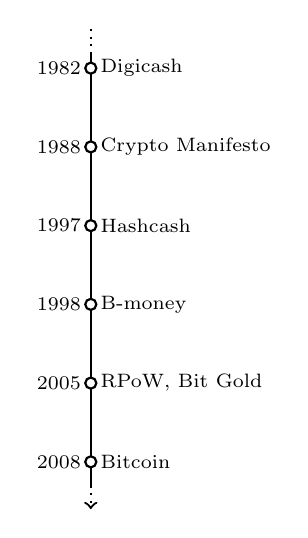
\begin{tikzpicture}[scale=1]
				%draw vertical line
		%\draw [thick] (0,4) -- (0,2.3);
		%\draw [thick,dotted] (0,2.3) -- (0,1.7);
		%\draw [thick] (0,1.7) -- (0,0.3);
		%\draw [thick,dotted] (0,0.3) -- (0,-0.3);
		%\draw [thick, ->] (0,-0.3) -- (0,-2);
		\draw [thick,dotted] (0,4) -- (0,3.7);
		\draw [thick] (0,3.7) -- (0,-1.8);
		\draw [thick,dotted, ->] (0,-1.8) -- (0,-2.1);
		
		%draw bullet points
		\foreach \x in {3.5,2.5,1.5,0.5,-0.5,-1.5}
		\filldraw[draw=black, fill = white, thick] (0, \x cm) circle (2pt);
		
		
		%years & names
		\draw(0,3.5) node[left] {{\scriptsize 1982}} node[right] {{\scriptsize Digicash}};
		\draw(0,2.5) node[left] {{\scriptsize 1988}} node[right] {{\scriptsize Crypto Manifesto}};
		\draw(0,1.5) node[left] {{\scriptsize 1997}} node[right] {{\scriptsize Hashcash}};
		\draw(0,0.5) node[left] {{\scriptsize 1998}} node[right] {{\scriptsize B-money}};
		\draw(0,-0.5) node[left] {{\scriptsize 2005}} node[right] {{\scriptsize RPoW, Bit Gold}};
		\draw(0,-1.5) node[left] {{\scriptsize 2008}} node[right] {{\scriptsize Bitcoin}};
	
	\end{tikzpicture}
\end{figure}
\column{0.7\textwidth}
	\textbf{Bit Gold - Nick Szabo}
	\vspace{0.5em}
	\begin{small}
	\begin{itemize}
		\item Describes the combination of the proof-of-work algorithm for competitive money creation.
		\item Computing power is used to collateralise a public ledger, which grows into a chain of blocks through a reflexive reference.
		\item "Thus, it would be very nice if there were a protocol whereby unforgeably costly bits could be created online with minimal dependence on trusted third parties, and then securely stored, transferred, and assayed with similar minimal trust. Bit gold."
	\end{itemize}
	\end{small}
\end{columns}
\end{frame}
%%%	


%%%
\begin{frame}{After Bitcoin: Forks and Altcoins}
	\begin{columns}
		\column{0.4\linewidth}
		\begin{figure}
			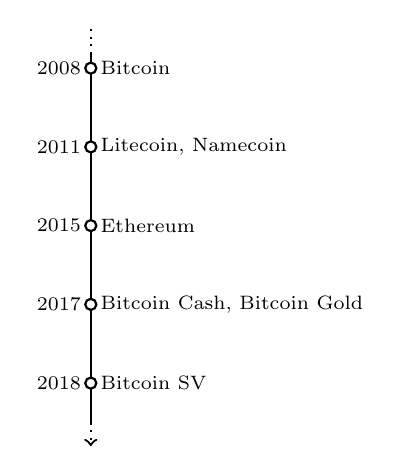
\begin{tikzpicture}[scale=1]
							%draw vertical line
		\draw [thick,dotted] (0,4) -- (0,3.7);
		\draw [thick] (0,3.7) -- (0,-1);
		\draw [thick, dotted, ->] (0,-1) -- (0,-1.3);

		%\draw [thick] (0,1.7) -- (0,0.3);
		%\draw [thick,dotted] (0,0.3) -- (0,-0.3);
		%\draw [thick, ->] (0,-0.3) -- (0,-2);
		
		%draw bullet points
		\foreach \x in {3.5,2.5,1.5,0.5,-0.5}
		\filldraw[draw=black, fill = white, thick] (0, \x cm) circle (2pt);
		
		
		%years & names
		\draw(0,3.5) node[left] {{\scriptsize 2008}} node[right] {{\scriptsize Bitcoin}};
		\draw(0,2.5) node[left] {{\scriptsize 2011}} node[right] {{\scriptsize Litecoin, Namecoin}};
		\draw(0,1.5) node[left] {{\scriptsize 2015}} node[right] {{\scriptsize Ethereum}};
		\draw(0,0.5) node[left] {{\scriptsize 2017}} node[right] {{\scriptsize Bitcoin Cash, Bitcoin Gold}};
		\draw(0,-0.5) node[left] {{\scriptsize 2018}} node[right] {{\scriptsize Bitcoin SV}};
		%\draw(0,-1.5) node[left] {{\scriptsize 2018}} node[right] {{\scriptsize Bitcoin SV}};
			\end{tikzpicture}
		\end{figure}
		\column{0.6\linewidth}
		\textbf{Litecoin}
		\vspace{0.5em}
		\begin{itemize}
			\item Based on Bitcoin Protocol
			\item Different hashing algorithm, Block time (2,5 min) and Hard Cap (84 million)
		\end{itemize}
		\vspace{0.5em}
		\textbf{Namecoin}
		\vspace{0.5em}
		\begin{itemize}
			\item Key/Value pair registration and transfer system based on the Bitcoin technology.
		\end{itemize}
	\end{columns}	
\end{frame}
%%%


%%%
\begin{frame}{After Bitcoin: Forks and Altcoins}
	\begin{columns}
		\column{0.4\linewidth}
		\begin{figure}
			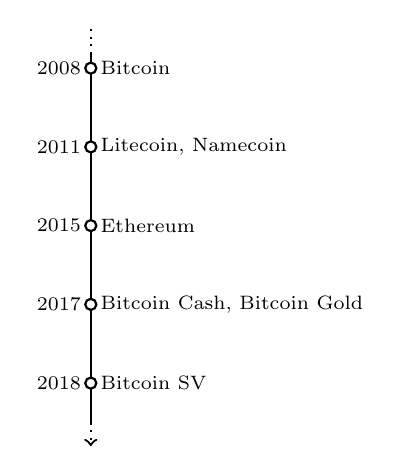
\begin{tikzpicture}[scale=1]
							%draw vertical line
		\draw [thick,dotted] (0,4) -- (0,3.7);
		\draw [thick] (0,3.7) -- (0,-1);
		\draw [thick, dotted, ->] (0,-1) -- (0,-1.3);

		%\draw [thick] (0,1.7) -- (0,0.3);
		%\draw [thick,dotted] (0,0.3) -- (0,-0.3);
		%\draw [thick, ->] (0,-0.3) -- (0,-2);
		
		%draw bullet points
		\foreach \x in {3.5,2.5,1.5,0.5,-0.5}
		\filldraw[draw=black, fill = white, thick] (0, \x cm) circle (2pt);
		
		
		%years & names
		\draw(0,3.5) node[left] {{\scriptsize 2008}} node[right] {{\scriptsize Bitcoin}};
		\draw(0,2.5) node[left] {{\scriptsize 2011}} node[right] {{\scriptsize Litecoin, Namecoin}};
		\draw(0,1.5) node[left] {{\scriptsize 2015}} node[right] {{\scriptsize Ethereum}};
		\draw(0,0.5) node[left] {{\scriptsize 2017}} node[right] {{\scriptsize Bitcoin Cash, Bitcoin Gold}};
		\draw(0,-0.5) node[left] {{\scriptsize 2018}} node[right] {{\scriptsize Bitcoin SV}};
		%\draw(0,-1.5) node[left] {{\scriptsize 2018}} node[right] {{\scriptsize Bitcoin SV}};
			\end{tikzpicture}
		\end{figure}
		\column{0.6\linewidth}
		\textbf{Ethereum - Vitalik Buterin}
		\vspace{0.5em}
		\begin{itemize}
			\item Protocol for building decentralized applications (dApps).
			\item Touring-complete scripting language $\rightarrow$ Smart Contracts
			\item Account based- instead of UTXO based model.
		\end{itemize}
	\end{columns}	
\end{frame}
%%%


%%%
\begin{frame}{Bitcoin Fork Timeline}
	\begin{figure}[h!]
	\center
		\begin{tikzpicture}[scale=0.65, every node/.style={scale=0.65}]
			\coordinate (o1) at (1,1);
\coordinate (o2) at (2,1);
\coordinate (o3) at (3,1);
\coordinate (o4) at (4,1);
\coordinate (o5) at (5,3);
\coordinate (o6) at (6,3);
\coordinate (o7) at (7,3);
\coordinate (o8) at (8,3);
\coordinate (o9) at (9,3);
\coordinate (o10) at (10,3);
\coordinate (o11) at (11,3);
\coordinate (o12) at (12,3);
\coordinate (o13) at (13,3);
\coordinate (o14) at (14,3);
\coordinate (o15) at (15,3);
\coordinate (o16) at (16,3);
\coordinate (o17) at (17,3);
\coordinate (n1) at (3,-2);
\coordinate (n2) at (4,-2);
\coordinate (n3) at (5,-2);
\coordinate (n4) at (6,-2);
\coordinate (n5) at (7,-2);
\coordinate (n6) at (8,-2);
\coordinate (n7) at (9,-2);
\coordinate (n8) at (10,-2);
\coordinate (n9) at (11,-2);
\coordinate (n10) at (12,-2);
\coordinate (n11) at (13,-2);
\coordinate (n12) at (14,-2);
\coordinate (s2) at (12,-4);
\coordinate (s3) at (13,-4);
\coordinate (x5) at (5,1);
\coordinate (z1) at (8,0.5);
\coordinate (z2) at (9,0.5);
\coordinate (z3) at (10,0.5);
\coordinate (z4) at (11,0.5);
\coordinate (z5) at (12,0.5);
\coordinate (z6) at (13,0.5);

  \node at (o1) [above=1em]{Bitcoin};
  \node at (n1) [below=1em]{B-Cash};
  \node at (o5) [above=1em]{Bitcoin (SegWit Update)};
  \node at (z1) [below=1em]{Bitcoin Gold};
  \node at (s2) [below=1em]{Bitcoin SV};

  \draw[] (o1) to[] (o2) to[] (o3) to[] (o4) to[] node[below, rotate=60]{\small{24.08.2017}}node[above, rotate=60]{\small{Softfork}}  (o5) to[] (o6) to[] (o7) to[] (o8) to[] (o9) to[] (o10) to[] (o11) to[] (o12) to[] (o13) to[] (o14) to[] (o15) to[] (o16) ;
  \draw[] (o2) to[] node [above, rotate=-75]{\small Forced Fork} node[below, rotate=-75]{\small{01.08.2017}} (n1)  to[] (n2) to[] (n3) to[] (n4) to[] (n5) to[] (n6) to[] (n7) to[] (n8) to[] (n9) to[] (n10) to[] (n11);
  \draw[] (n9) to[] node [above, rotate=-65]{\small Forced Fork} node[below, rotate=-65]{\small{15.11.2018}} (s2) ;
  \draw[] (o4) to[] (x5) ;
  \draw[] (o7) to[] node [above, rotate=-67]{\small Forced Fork} node[below, rotate=-67]{\small{24.10.2017}} (z1) ;
  \draw[] (z1) to[] (z2) to[] (z3) to[] (z4) to[] (z5);
  %\draw[color=black] (n6) to[] (o7);
  %\draw[color=black,densely dashed] (o4) to[] (o5);
  %\draw[color=black,densely dashed] (o7) to[] (o8);
  \draw[color=black,thick, dotted, ->] (o16) to[] (o17);
  \draw[color=black,thick, dotted, ->] (n11) to[] (n12);
  \draw[color=black,thick, dotted, ->] (s2) to[] (s3);  
  \draw[color=black,thick, dotted, ->] (z5) to[] (z6);  

  %\filldraw[draw=black,fill=white] (o1) circle (5pt);
  %\filldraw[draw=black,fill=white] (o2) circle (5pt);
  %\filldraw[draw=black,fill=white] (o3) circle (5pt);
  %\filldraw[draw=black,fill=white] (o4) circle (5pt);
  %\filldraw[draw=black,fill=white] (o5) circle (5pt);
  %\filldraw[draw=black,fill=white] (o6) circle (5pt);
  %\filldraw[draw=black,fill=white] (o7) circle (5pt);
  %\filldraw[draw=black,fill=white] (o8) circle (5pt);
  %\filldraw[draw=black,fill=white] (o9) circle (5pt);
  \node (rect) at (o1) [fill=highlight,draw,minimum width=0.3cm,minimum height=0.3cm] {};
  \node (rect) at (o2) [fill=highlight,draw,minimum width=0.3cm,minimum height=0.3cm] {};
  \node (rect) at (o3) [fill=highlight,draw,minimum width=0.3cm,minimum height=0.3cm] {};
  \node (rect) at (o4) [fill=highlight,draw,minimum width=0.3cm,minimum height=0.3cm] {};
  \node (rect) at (o5) [fill=highlight,draw,minimum width=0.3cm,minimum height=0.3cm] {};
  \node (rect) at (o6) [fill=highlight,draw,minimum width=0.3cm,minimum height=0.3cm] {};
  \node (rect) at (o7) [fill=highlight,draw,minimum width=0.3cm,minimum height=0.3cm] {};
  \node (rect) at (o8) [fill=highlight,draw,minimum width=0.3cm,minimum height=0.3cm] {};
  \node (rect) at (o9) [fill=highlight,draw,minimum width=0.3cm,minimum height=0.3cm] {};
  \node (rect) at (o10) [fill=highlight,draw,minimum width=0.3cm,minimum height=0.3cm] {};
  \node (rect) at (o11) [fill=highlight,draw,minimum width=0.3cm,minimum height=0.3cm] {};
  \node (rect) at (o12) [fill=highlight,draw,minimum width=0.3cm,minimum height=0.3cm] {};
  \node (rect) at (o13) [fill=highlight,draw,minimum width=0.3cm,minimum height=0.3cm] {};
  \node (rect) at (o14) [fill=highlight,draw,minimum width=0.3cm,minimum height=0.3cm] {};
  \node (rect) at (o15) [fill=highlight,draw,minimum width=0.3cm,minimum height=0.3cm] {};
  \node (rect) at (o16) [fill=highlight,draw,minimum width=0.3cm,minimum height=0.3cm] {};
  %\filldraw[draw=black,fill=highlight] (n4) circle (5pt);
  %\filldraw[draw=black,fill=highlight] (n5) circle (5pt);
  %\filldraw[draw=black,fill=highlight] (n6) circle (5pt);
  %\filldraw[draw=black,fill=highlight] (n7) circle (5pt);
  %\filldraw[draw=black,fill=highlight] (n8) circle (5pt);
  %\filldraw[draw=black,fill=highlight] (n9) circle (5pt);
  \node (rect) at (n1) [fill=white,draw,minimum width=0.3cm,minimum height=0.3cm] {};
  \node (rect) at (n2) [fill=white,draw,minimum width=0.3cm,minimum height=0.3cm] {};
  \node (rect) at (n3) [fill=white,draw,minimum width=0.3cm,minimum height=0.3cm] {};
  \node (rect) at (n4) [fill=white,draw,minimum width=0.3cm,minimum height=0.3cm] {};
  \node (rect) at (n5) [fill=white,draw,minimum width=0.3cm,minimum height=0.3cm] {};
  \node (rect) at (n6) [fill=white,draw,minimum width=0.3cm,minimum height=0.3cm] {};
  \node (rect) at (n7) [fill=white,draw,minimum width=0.3cm,minimum height=0.3cm] {};
  \node (rect) at (n8) [fill=white,draw,minimum width=0.3cm,minimum height=0.3cm] {};
  \node (rect) at (n9) [fill=white,draw,minimum width=0.3cm,minimum height=0.3cm] {};
  \node (rect) at (n10) [fill=white,draw,minimum width=0.3cm,minimum height=0.3cm] {};
  \node (rect) at (n11) [fill=white,draw,minimum width=0.3cm,minimum height=0.3cm] {};
  %\node (rect) at (s1) [fill=white,draw,minimum width=0.3cm,minimum height=0.3cm] {};
  \node (rect) at (s2) [fill=white,draw,minimum width=0.3cm,minimum height=0.3cm] {};
  \node (rect) at (x5) [fill=white,draw,minimum width=0.3cm,minimum height=0.3cm] {};
  \node (rect) at (z1) [fill=white,draw,minimum width=0.3cm,minimum height=0.3cm] {};
  \node (rect) at (z2) [fill=white,draw,minimum width=0.3cm,minimum height=0.3cm] {};
  \node (rect) at (z3) [fill=white,draw,minimum width=0.3cm,minimum height=0.3cm] {};
  \node (rect) at (z4) [fill=white,draw,minimum width=0.3cm,minimum height=0.3cm] {};
  \node (rect) at (z5) [fill=white,draw,minimum width=0.3cm,minimum height=0.3cm] {};
  		\end{tikzpicture}
		%\caption{Bitcoin fork timeline.}
		\label{fig:forkhistory}
	\end{figure}
\end{frame}
%%%


%%%
\begin{frame}{Bitcoin as Money?}
	\begin{figure}
		\begin{tikzpicture}
		\begin{footnotesize}
	
		\draw[dotted, above] (0,0) rectangle (9.6, 1.3) node[above = 3pt, midway] (Unit) {\textbf{Monetary unit}};
		
		\alert<1>{
		\uncover<1->{\filldraw[fill = highlight, draw = highlight!20!black] (0.2, 0.1) rectangle (3.2, 0.8) node[midway] {Medium of exchange};}
		}
		\alert<2>{
		\uncover<2->{\filldraw[fill = highlight, draw = highlight!20!black] (3.3, 0.1) rectangle (6.3, 0.8) node[midway] {Unit of account};}
		}
		\alert<3>{
		\uncover<3->{\filldraw[fill = highlight, draw = highlight!20!black] (6.4, 0.1) rectangle (9.4, 0.8) node[midway] {Store of value};}
		}
		\end{footnotesize}
		\end{tikzpicture}
	\end{figure}
	\begin{itemize}
			\item<1-> Due to comparatively low adoption rates and technical limitations, Bitcoin falls short of becoming the dominant medium of exchange at the moment.
			\item<2-> People have certain difficulties in grasping decimal numbers and interpreting their information content correctly.
			\item<3-> Relatively high volatility (speculation, capped supply). More confidence should lower volatility, but will probably settle at a high level compared to other monetary units.
	\end{itemize}
\end{frame}
%%%


%%%
\begin{frame}%[allowframebreaks]
\frametitle{References and Recommended Reading}
	\bibliographystyle{amsplain}
	\bibliography{../assets/bib/refs}
\end{frame}

\end{document}

%%%
%\begin{frame}{Before Bitcoin}

%\begin{figure}
%	\begin{tikzpicture}[scale=1]
	
	%draw horizontal line
%	\draw [thick] (0,0) -- (3,0);
%	\draw [thick,dotted] (3.1,0) -- (3.7,0);
%	\draw [thick, ->] (3.7,0) -- (10,0);
	%draw vertical lines
%	\foreach \x in {0.66,2.66,4.11,5,7.33,9.33}
%	\draw (\x cm, 3pt) -- (\x cm, -3pt);
	
	%years
%	\draw[ultra thick] (0.66,0) node[above=3pt] {{\scriptsize 1982}} ;
%	\draw[ultra thick] (2.66,0) node[above=3pt] {{\scriptsize 1988}} ;
%	\draw[ultra thick] (4.11,0) node[above=3pt] {{\scriptsize 1997}} ;
%	\draw[ultra thick] (5,0) node[above=3pt] {{\scriptsize 1998}} ;
%	\draw[ultra thick] (7.33,0) node[above=3pt] {{\scriptsize 2005}} ;
%	\draw[ultra thick] (9.33,0) node[above=3pt] {{\scriptsize 2008}} ;	
	
		%years
%	\draw[ultra thick] (0.66,0) node[below=3pt] {{\scriptsize Digicash}} ;
%	\draw[ultra thick] (2.66,0) node[below=3pt] {{\scriptsize Crypto Manifesto}} ;
%	\draw[ultra thick] (4.11,0) node[below=3pt] {{\scriptsize Hashcash}} ;
%	\draw[ultra thick] (5,0) node[below=3pt] {{\scriptsize b-money}} ;
%	\draw[ultra thick] (7.33,0) node[below=3pt] {{\scriptsize Bit Gold}} ;
%	\draw[ultra thick] (9.33,0) node[below=3pt] {{\scriptsize 2008}} ;	
	
	%Text
	%\node[align=center] at (0.5,-1.2) {{\scriptsize Digicash}};
	
	%\node[align=center] at (2.66,1) {{\scriptsize Crypto Manifesto}};
	
	%\node[align=center] at (4.11,-1.2) {{\scriptsize Hashcash}};
	
	%\node[align=center] at (5,1) {{\scriptsize B-money}};
	
	%\node[align=center] at (7.33,-1.2) {{\scriptsize Reusable Proofs of Work}};
	
	%\node[align=center] at (7.33,0.7) {{\scriptsize Bit Gold}};
	
	%\node[align=center] at (9.33,0.7) {{\scriptsize Bitcoin}};
	
	%\end{tikzpicture}
%\end{figure}
%\end{frame}
%%%
